\documentclass[a4paper]{article}

%use the english line for english reports
%usepackage[english]{babel}
\usepackage[portuguese]{babel}
\usepackage[utf8]{inputenc}
\usepackage{indentfirst}
\usepackage{graphicx}
\usepackage{verbatim}
\usepackage{fancyhdr}

\pagestyle{fancy}
\fancyhf{}
\renewcommand{\headrulewidth}{0pt}
\fancyhead{}
\fancyfoot[R]{\thepage}


\begin{document}

\setlength{\textwidth}{16cm}
\setlength{\textheight}{22cm}

\title{\Huge\textbf{Blockade}\linebreak\linebreak\linebreak
\Large\textbf{Relatório Final}\linebreak\linebreak
\linebreak\linebreak

\includegraphics[scale=0.1]{feup-logo.png}\linebreak\linebreak
\linebreak\linebreak
\Large{Mestrado Integrado em Engenharia Informática e Computação} \linebreak\linebreak
\Large{Programação em Lógica}\linebreak
}

\author{\textbf{Grupo:}\\  João Barbosa - up201406241 \\ José Martins - up201404189 \\\linebreak\linebreak \\
 \\ Faculdade de Engenharia da Universidade do Porto \\ Rua Roberto Frias, s\/n, 4200-465 Porto, Portugal 
\vspace{1cm}}
\date{12 de Novembro de 2016}
\maketitle
\thispagestyle{empty}

%************************************************************************************************
%************************************************************************************************

\newpage

\section*{Resumo}
No âmbito da unidade curricular "Programação em Lógica" do 3º ano do Mestrado Integrado em Engenharia Informática e Computação, da Faculdade de Engenharia da Universidade do Porto, foi proposto o desenvolvimento de um jogo de tabuleiro, utilizando a linguagem \textit{Prolog}. O jogo  escolhido denomina-se \textbf{Blockade}. \par
A utilização de \textit{Prolog}, uma linguagem do paradigma da programação lógica, mostrou-se não só interessante, pois foi possível perceber as grandes potencialidades e vantagens da linguagem, como também desafiante, devido à inexperiência neste tipo de paradigma. \par
Para o desenvolvimento do projeto, foi necessário perceber e estruturar os conceitos-chave do jogo, de forma a obter a melhor forma de proceder à implementação do jogo. Além disso, foi necessário aprofundar o conhecimento sobre as bibliotecas disponibilizadas pela linguagem, para garantir qualidade e segurança no código. \par
O resultado final da implementação do jogo mostra-se como uma boa reprodução do \textbf{Blockade}. Adicionalmente, permite que os jogadores sejam \mbox{\textbf{humanos}} (que escolhem as jogadas que pretendem fazer), ou \textbf{\textit{bots}} (que avaliam a melhor jogada que podem executar).

\newpage

\tableofcontents

%************************************************************************************************
%************************************************************************************************

%*************************************************************************************************
%************************************************************************************************

\newpage

%%%%%%%%%%%%%%%%%%%%%%%%%%
\section{Introdução}


Este trabalho foi desenvolvido no âmbito da unidade curricular “Programação em Lógica” do 3º ano do Mestrado Integrado em Engenharia Informática e Computação da Faculdade de Engenharia da Universidade do Porto. O seu objetivo é o de implementar em Prolog um jogo de tabuleiro de 2 jogadores de forma a possibilitar o jogo Humano vs. Humano, Humano vs. Computador e Computador vs. Computador.
Neste relatório será descrito o jogo que escolhemos para a nossa implementação – o “Blockade” – assim como as suas regras. De seguida, serão detalhadas algumas funcionalidades e características da nossa implementação, desde a representação do jogo e visualização do tabuleiro até a avaliação de jogadas pelo computador e final do jogo. Por fim, serão apresentadas as conclusões que obtivemos da realização deste trabalho, bem como a sua bibliografia.



%%%%%%%%%%%%%%%%%%%%%%%%%%
\newpage
\section{O Jogo Blockade}

Blockade trata-se de um jogo de tabuleiro produzido pela primeira vez em 1975 pela Lakeside Games.
O jogo é desenhado para 2 jogadores sendo que cada um possui: 

\begin{itemize}
\item 2 Peões
\item 9 Parede verdes (que só podem ser colocadas verticalmente)
\item 9 Paredes azuis (que só podem ser colocadas horizontalmente)
\end{itemize}

O tabuleiro do jogo é um quadriculado com dimensões 11x14, com 2 pontos amarelos e dois pontos laranja que representam a base, e as posições iniciais, dos dois peões de cada jogador. Estes pontos distam 4 quadrículas de cada canto na diagonal. 

\begin{center}
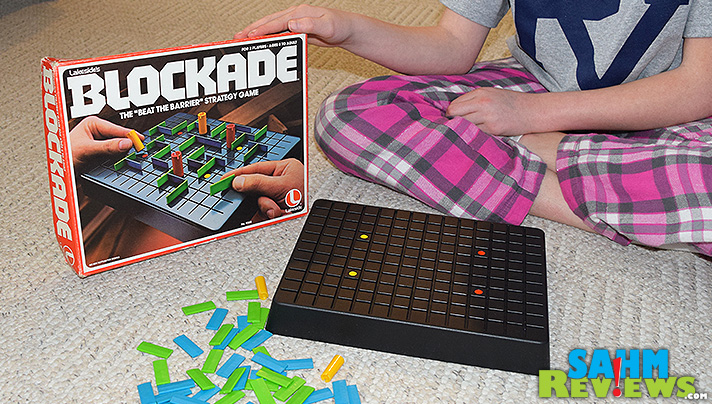
\includegraphics[scale = 0.3]{fig1.jpg}
\end{center}

Trata-se de um jogo de turnos, em que em cada turno um jogador pode mover um dos seus peões, uma ou duas quadrículas (horizontalmente, verticalmente ou uma combinação das duas), e posicionar uma parede de modo a tentar bloquear os movimentos do adversário.
As paredes ocupam sempre duas quadrículas e devem ser posicionadas de acordo com a sua cor. Peões podem saltar por cima de outros peões que estejam a bloquear o seu caminho.
O objetivo do jogo é levar um dos seus peões até à base de um dos peões do adversário. Quando os jogadores ficarem sem paredes para colocar, continuam a mover-se até que alguém vença o jogo. 

\begin{center}
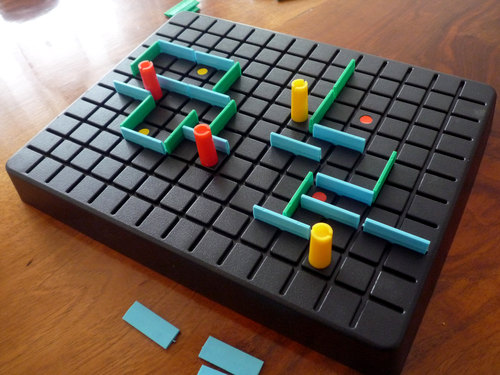
\includegraphics[scale = 0.4]{fig2.jpg}
\end{center}

%%%%%%%%%%%%%%%%%%%%%%%%%%
\section{Lógica do Jogo}


\subsection{Representação do Estado do Jogo} 

O jogo possui uma representação interna, utilizada para o processamento e armazenamento de informação, e uma representação externa, para tornar a visualização do jogo mais apelativa e intuitiva. A simbologia utilizada é a seguinte: 


\begin{center}
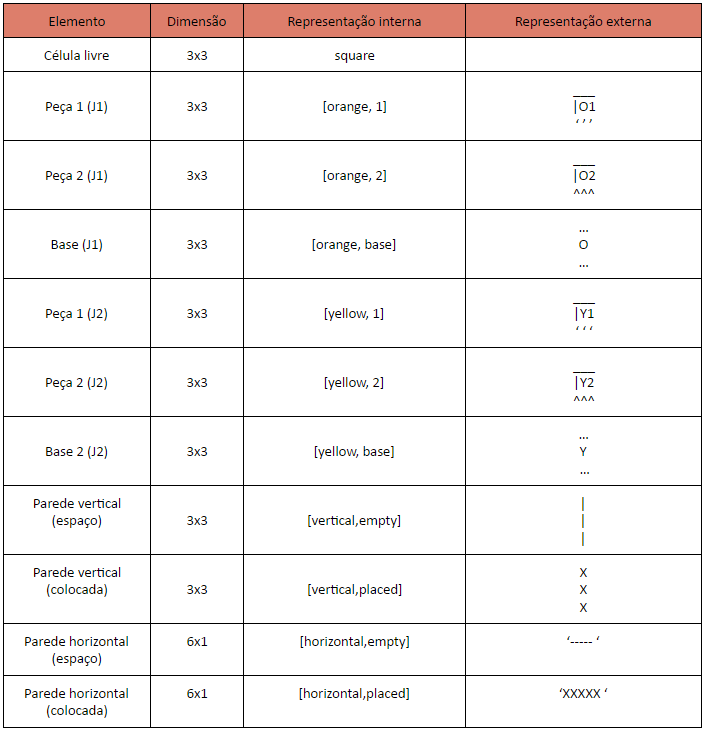
\includegraphics[scale = 0.7]{fig3.png}
\end{center}

O tabuleiro é tambem representado internamente por um grafo, de modo a permitir a utilização de algoritmos de  'Path Finding' na avaliação das melhores jogadas e em algumas verificações.

%%%%%%%%%%%%%%%%%%%%%%%%%%
\newpage
\subsection{Visualização do Tabuleiro} 
O tabuleiro será visualizado através da utilização de caracteres ASCII para representar os peãos, paredes e bases de cada jogagor, exemplo:


\begin{center}
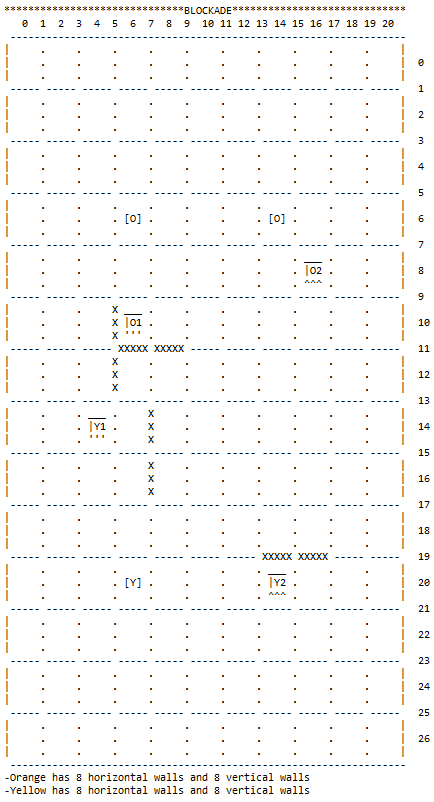
\includegraphics[scale = 0.7]{fig4.png}
\end{center}


\subsection{Lista de Jogadas Válidas} 

As jogadas são obtidas através do input do jogador ou através dos algoritmos implementados para permitir o calculo da jogada do computador, sendo posteriormente verificada a sua validade.

%%%%%%%%%%%%%%%%%%%%%%%%%%
\newpage
\subsection{Execução de Jogadas} 

Depois de obtidas as coordenadas para a movimentação do jogador é utilizado o predicado \textit{validPosition(+Pawn,+ Board, +X,+ Y,-Nx,-Ny)}, este predicado recebe o offset (X,Y) para onde o jogador se quer mover em relação á sua posição atual e falha quando as coordenadas finais da ''futura'' posição do jogador se encontram fora das dimensões do tabuleiro ou quando existe uma parede a bloquear a movimentação para as novas coordenadas.
\par Assim que a jogada se encontra validada é chamado o predicado \textit{moveOneSpace(+Pawn, +X, +Y, +Board, -NewBoard)}, que move o peão num offset (X,Y) criando um novo tabuleiro.
\par Existe tambem outro predicado para validar e posicionar as paredes, este denomina-se \textit{placeWall(+Player,+X,+ Y,+O,+Board, -NewBoard)},  o predicado é bem sucedido quando as coordenadas da parede são validas, criando assim um novo tabuleiro.
\par No entanto o predicado fallha quando as coordenadas são invalidas devido a um dos motivos:
\begin{itemize}
	\item A parede está para lá dos limites do tabuleiro
	\item A parede está cruzada com outra parede
	\item A parede bloqueia completamente o jogador (ou seja quando o posicionamento da parede impossibilita que um dos peões deixe de ter um caminho para as bases adversárias)
\end{itemize}

Estes predicados podem ser encontrados no ficheiro board/logic.pl.



\subsection{Avaliação do Tabuleiro} Na nossa implementação, não existe uma avaliação direta do tabuleiro, para comparar as diferentes jogadas possíveis, pois:
\begin{itemize}
	\item Quando o jogador é um humano, a direção do movimento é pedida via linha de comandos. Neste contexto, a avaliação da jogada é ignorada, pois o jogador deve ter liberdade para a fazer, independentemente da sua qualidade.
	
	\item Quando o jogador é um computador em nível fácil, os movimentos são aleatórios, não havendo qualquer avaliação do tabuleiro.
	
	\item Quando o jogador é um computador em nível difícil, a movimentação das peças é feita com recurso a \textit{pathfinding}, que nos devolve a melhor jogada possível. \\
Este algoritmo avalia internamente o grafo, e determina qual o caminho de menor custo para o jogador. Esta avaliação do tabuleiro é indireta, visto que os algoritmos sobre grafos utilizados estão implementados nas biliotecas do \textit{Prolog}.
\end{itemize}


%%%%%%%%%%%%%%%%%%%%%%%%%%
\newpage
\subsection{Final do Jogo} A verificação de que o jogo chegou ao fim é testada usando o predicado \mbox{\textit{checkEnd}}. Este predicado não precisa de argumentos, pois as posições dos jogadores são extraídas diretamente da base de dados, utilizando o predicado auxiliar \textit{position(+Player, -X, -Y)}. \par
Se alguns dos jogadores chegar ao seu objetivo, i.e. a uma das bases do oponente, então o predicado retorna \textit{true}, e, consequentemente, termina o ciclo de jogo.




\subsection{Jogada do Computador} 

Foram implementados dois niveis de dificuldade para a jogada do computador:

\textbf{Nivel Fácil}
\begin{itemize}
\item Este modo é totalmente aleatório, desta forma não realiza nenhuma consideração sobre o estado de jogo. Para criar a jogada são utilizados os predicados:
	\begin{itemize}
		\item \textit{randomMove(-X, -Y)} - para calcular uma movimentação aleatória.
		\item \textit{randomWall(-X, -Y, -O)} - para calcular uma parede aleatória.
	\end{itemize}
	 Quando as coordenadas devolvidas não são validas, os predicados voltam a ser executados, até ser encontrada uma jogada possivel.
\end{itemize}

\textbf{Nivel Difícil}
\begin{itemize}
\item Este modo procura a melhor jogada possivel no momento, utilizando ''path finding'' para encontrar o caminho mais curto tendo em consideração todas as paredes já posicionadas, assim é escolhido de entre os dois peões do jogador o melhor a ser movido e a melhor direção para o mover.
No que diz respeito ás paredes, é feito o processo contrário ou seja o predicado determina o melhor peão do oponente e a melhor direção para ele se movimentar tentando depois colocar uma parede a bloquea-lo, se não for possivel colocar a parede a bloquear a melhor direção do melhor peão do oponente é escolhida outra parede, de modo a bloquea-lo noutra direção.
 Para criar a jogada neste nivel são utilizados os predicados:
 \begin{itemize}
		\item \textit{evaluateBestPawn(+Player,-N)} - para calcular o melhor peão a movimentar.
		\item \textit{evaluateBestDirectionPro(+Player,+Id, -Direction)}-  para calcular a melhor direção para o peão.
		\item \textit{evaluateBestWall(+Player,-Walls)}- para calcular uma lista ordenada com as melhores paredes a posicionar para bloquear o oponente de Player.
	\end{itemize}
\end{itemize}







%%%%%%%%%%%%%%%%%%%%%%%%%%
\newpage
\section{Interface com o Utilizador}


Foram criados diversos menus para permitir uma fácil interação do utilizador com o programa.
\par As opções possiveis estão sempre explicitas nos menus, o utilizador deverá colocar um '.' a seguir á opção pretendida  (ex. '1.').
\par Aquando da chamada do predicado \textit{blockade} (sem argumentos) o jogo iniciasse, sendo mostrado ao utilizador o seguinte menu.

\begin{center}
	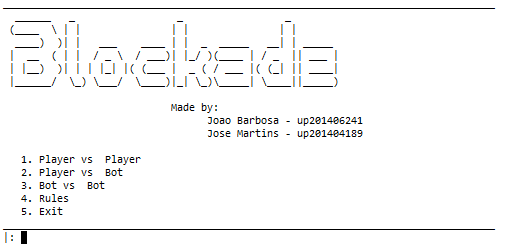
\includegraphics[scale = 0.7]{fig5.png}
\end{center}

Se a escolha do utilizador passar pela opção 2 ou 3 é apresentado o seguinte menu, para permitir a seleção da diculdade pretendida.

\begin{center}
	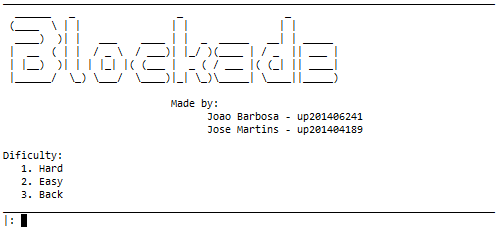
\includegraphics[scale = 0.7]{fig6.png}
\end{center}

Em ambiente de jogo é representado o tabuleiro atual e no fim deste são apresentados os dialogos correspondentes á ação a ser tomada no momento.

  \begin{itemize}
		\item Diálogo para a movimentação de um peão do jogador.	
		\begin{center}
			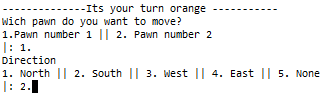
\includegraphics[scale = 0.7]{fig7.png}
		\end{center}
		\item Diálogo para a colocação de uma parede.
		\begin{center}
			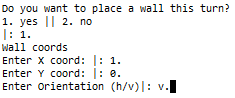
\includegraphics[scale = 0.7]{fig8.png}
		\end{center}
	\end{itemize}






%%%%%%%%%%%%%%%%%%%%%%%%%%
\section{Conclusões}
Tendo em conta resultado final da implementação, é possível afirmar que os principais objetivos deste projeto foram cumpridos:
\begin{itemize}
	\item Reprodução completa do jogo \textbf{Blockade}.
	\item Modos de jogo \texttt{Humano vs Humano}, \texttt{Humano vs Computador}, \texttt{Computador vs Computador}.
	\item Dois níveis de inteligência para o \textbf{\textit{bot}}.
	\item Interface com o utilizador
\end{itemize}
\ \par
Durante o desenvolvimento, foi possível perceber as potencialidades do \textit{Prolog}, e as vantagens de utilizar programação em lógica: a codificação das operações de natureza puramente lógica tornam-se mais intuitivas de realizar, e a implementação de certos algoritmos é facilitada pela natureza da linguagem. \\
É também de notar que o \textit{Prolog} possui muitas bibliotecas que podem ajudar a construir código com qualidade e segurança e, por esse motivo, foram utilizadas sempre que fossem convenientes. \par
No entanto, é importante reconhecer que, devido à inexperiência na linguagem, algumas implementações poderiam ser melhoradas. Especificamente, o tabuleiro de jogo possui 2 representações internas: uma em lista de listas, e outra em grafo. Isto acontece porque a representação inicial utilizada foi lista de listas, mas devido ao \textit{pathfinding}, foi também necessário a criação de um grafo. \par
As duas representações foram mantidas porque:
\begin{itemize}
	\item A maioria dos predicados utiliza a representação em lista de listas.
	\item O \textit{refactor} dos mesmos predicados seria custoso, em termos de tempo.
	\item A utilização única de representação em grafo provocaria algum \textit{overhead} em certas componentes (p.ex no \textit{display} do tabuleiro).
\end{itemize}
No entanto, esta solução apresenta algumas desvantagens:
\begin{itemize}
	\item Ocupa mais espaço em memória.
	\item A atualização do tabuleiro ocorre em dois sítios.
\end{itemize}
Um maior conhecimento prévio do \textit{Prolog}, e das bibliotecas que oferece, preveniria este acontecimento. \\ \par
Concluímos, portanto, que este projeto possibilitou a aprendizagem e consolidação de um novo tipo de paradigma de programação, abrindo novos horizontes e novas possibilidades, na definição e implementação de soluções para novos problemas.


\clearpage
\addcontentsline{toc}{section}{Bibliografia}
\renewcommand\refname{Bibliografia}
\bibliographystyle{plain}
\bibliography{myrefs}

\newpage
\appendix
\section{Anexo Código}
Código Prolog implementado devidamente comentado e outros elementos úteis que não sejam essenciais ao relatório.

\end{document}
